\chapter{Статические магнитоэлектрические эффекты}\label{ch:ch2}

В данной главе анализируются экспериментальные данные по магнитоэлектрической связи ионов меди и никеля в \ncbo, полученные в работах \cite{Nenert2007, Khan2013} (см. \cref{sec:ch1/sec2}). Объясняется, почему авторы \cite{Nenert2007} не смогли обнаружить индукции электрической поляризации при переходе чистого \cbo\ в антиферромагнитную фазу и почему это удалось сделать в соединении, допированном ионами \niIon.

\section{Расчет расщепления состояний \cud\ и \nif\ кристаллическим полем}\label{sec:ch2/sec1}

Эффективность рассматриваемого нами далее механизма зависит от особенностей энергетической структуры магнитного иона. Согласно структурным данным \cite{Martinez1971}, магнитные ионы \niIon и \cu занимают позиции с точечной группой симметрии \(S_4\) (рис. \cref{fig:cu_distributions}).

\begin{figure}[ht]
    \centerfloat{
        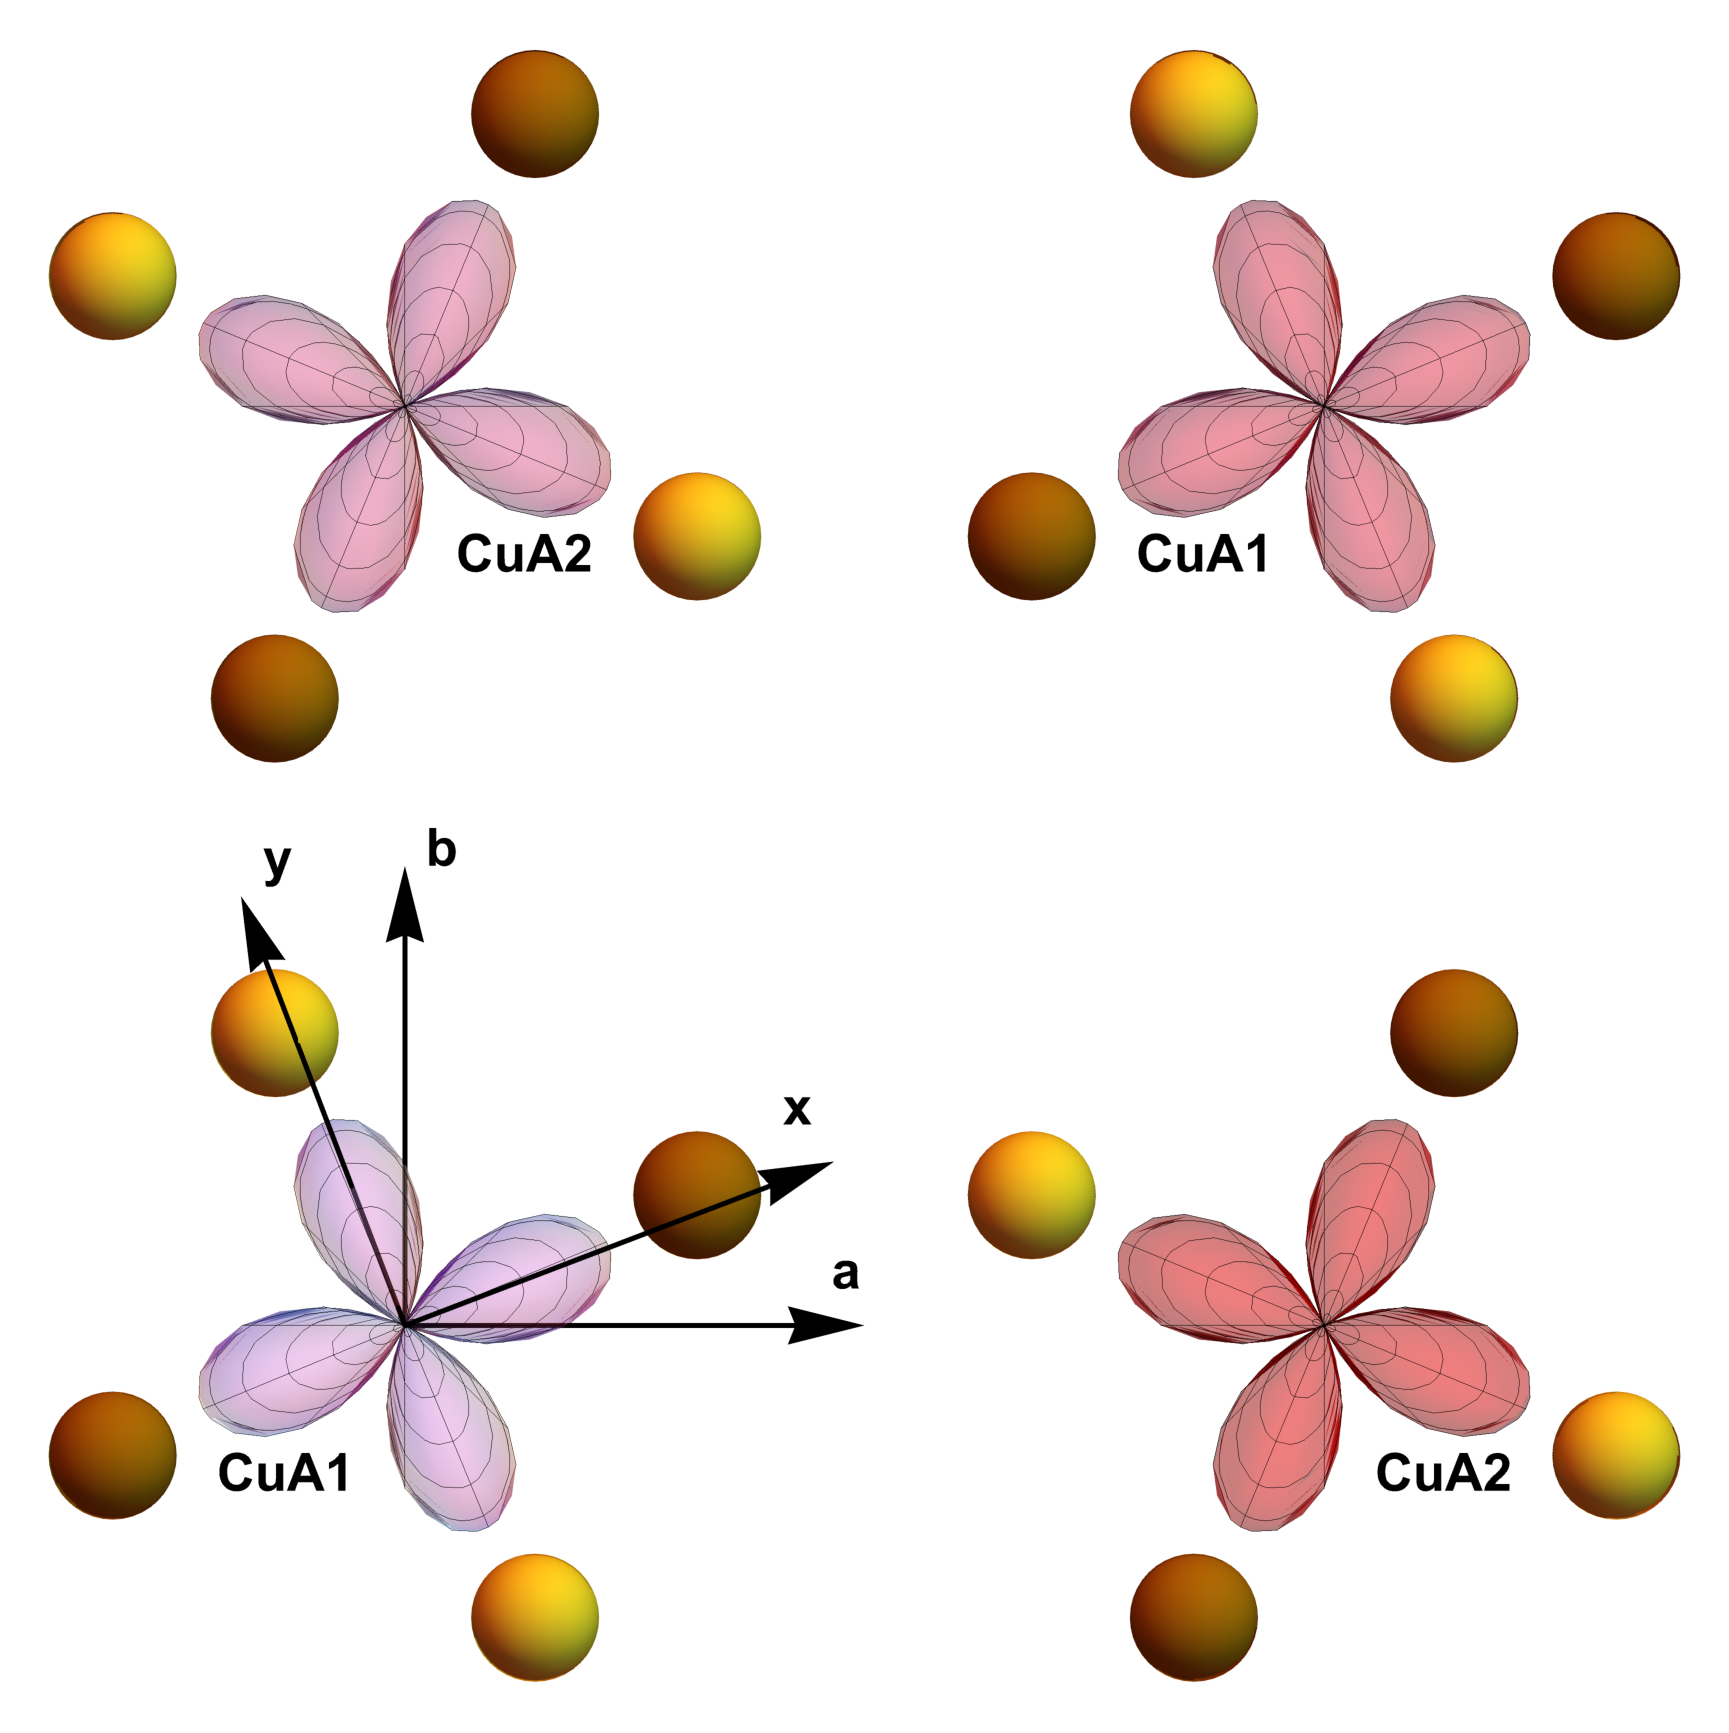
\includegraphics[scale=0.4]{cu_distributions}
    }
    \caption{Ортографическая проекция позиций элементарной ячейки подрешетки Cu 4b. Светло- и темно- желтым цветом изображены ионы кислорода, находящиеся соответственно выше и ниже по оси \textbf{c} относительно иона меди. Лепестки – рассчитанные нами распределения электронной плотности основных состояний ионов меди. \textit{a} и \textit{b} --- оси кристаллографической системы координат, \textit{x} и \textit{y} --- локальной оси локальной системы координат позиции A1. Насыщенность красного цвета в распределении электронной плотности меди соответствует увеличению координаты $z$ вдоль оси \textbf{c}, т.е. значениям $z\,{=}\,0,\,0.25,\,0.5 \text{ и } 0.75$ в единицах постоянных решетки в порядке увеличения яркости. Масштаб расстояний между позициями меди не соблюден.}\label{fig:cu_distributions}
\end{figure}

В этом случае оператор кристаллического поля имеет вид:

\begin{equation}
	\label{eq:Hcf}
	H_{cf}=B_{0}^{(2)}C_{0}^{(2)}+B_{0}^{(4)}C_{0}^{(4)}+B_{4}^{(4)}C_{4}^{(4)}+B_{-4}^{(4)}C_{-4}^{(4)},
\end{equation}

где $C_{q}^{(k)}$ - компоненты сферических тензорных операторов кристаллического поля, действующих на состояния 3d-электронов. Они связаны со сферическими функциями $Y_{k,q}\left( \theta,\phi \right)$ соотношением: $C_{q}^{(k)}=\sqrt{\frac{4\pi}{2k+1}}\sum Y_{k,q}\left( \theta_{i},\phi_{i} \right)$. Индекс суммирования $i$ относится к электронам в 3d-оболочке.

Ввиду того, что оба иона (\cu\ и \niIon) имеют одинаковый заряд, а при замещении меди никелем параметры кристаллической структуры в пределах погрешности не изменяются \cite{Khan2013}, эти ионы имеют общий набор параметров кристаллического поля.
Эти параметры $B_{q}^{(k)}$ рассчитывались нами с использованием модели обменных зарядов \cite{Malkin1987}. Для оценки обменного заряда на связях никель-кислород привлекались экспериментальные данные о кристаллических расщеплениях \cu\ в \cbo, полученные в работе \cite{Pisarev2011}. Наша теоретико-групповая интерпретация возбужденных состояний соответствует интерпретации, предложенной Меньшениным \cite{Menshenin2017}. В локальной системе координат они оказались равными (в см$^{-1}$):

\begin{equation}
	\label{eq:CrystParams}
	B_{0}^{(2)}=-17720, B_{0}^{(4)}=9940, B_{4}^{(4)}=14030.
\end{equation}

Локальная система координат выбиралась из условия $Im\left[ B_{4}^{(4)} \right]=0$ и $Re\left[ B_{4}^{(4)} \right]>0$ --- для того, чтобы матрица оператора \cref{eq:Hcf} имела диагональный вид. Это означает, что для позиции \textit{A1} локальная система координат повернута относительно кристаллографической системы на угол \ang{20.9} вокруг оси с кристалла (угол отсчитывается против часовой стрелки), для позиции \textit{A2} угол поворота, соответственно равен минус \ang{20.9}. Интересно, что эти направления не совпадают с направлениями на соседние ионы кислорода из-за действия оинов более удаленных координационных сфер. Энергии кристаллических подуровней основного терма \cud\ и \nif\ и соответствующие им волновые функции приведены в таблицах \cref{tab:NiEnAndWf} и \cref{tab:CuEnAndWf} соответственно.

\begin{table} [htbp]% Пример записи таблицы с номером, но без отображаемого наименования
	\centering
	\begin{threeparttable}% выравнивание подписи по границам таблицы
		\caption{Уровни энергии и волновые функции \niIon\ в \nbo.}%
		\label{tab:NiEnAndWf}%
		\begin{SingleSpace}
			\begin{tabular}{| c | c | c |}
				\hline 
				Уровни энергии & Представления точечной & \multirow{2}{*}{Волновые функции} \\ 
				в см$^{-1}$ & группы $\mathrm{S}_{4}$ &  \\ 
				\hline 
				\multirow{2}{*}{13943} & \multirow{2}{*}{${ }^{2} \Gamma_{34}$} & $\psi_{7}=\mathrm{C}_{2}|-1\rangle+\mathrm{C}_{1}|3\rangle$ \\
				& & $\psi_{6}=\mathrm{C}_{2}|1\rangle+\mathrm{C}_{1}|-3\rangle$ \\
				\hline
				13768 & $\phantom{{ }^{2} }\Gamma_{1\phantom{4}}$ & $\psi_{5}=|0\rangle$ \\
				\hline
				11179 & ${ }^{2} \Gamma_{2\phantom{4}}$ & $\psi_{4}=\frac{1}{\sqrt{2}}(|2\rangle+|-2\rangle)$ \\
				\hline
				\multirow{2}{*}{4744} & \multirow{2}{*}{${ }^{1} \Gamma_{34}$} & $\psi_{3}=\mathrm{C}_{1}|-1\rangle-\mathrm{C}_{2}|3\rangle$ \\
				& & $\psi_{2}=\mathrm{C}_{1}|1\rangle-\mathrm{C}_{2}|-3\rangle$ \\
				\hline 0 & ${ }^{1} \Gamma_{2\phantom{4}}$ & $\psi_{1}=\frac{1}{\sqrt{2}}(|2\rangle-|-2\rangle)$ \\
				\hline
			\end{tabular}%
		\end{SingleSpace}
	\end{threeparttable}
\end{table}

\begin{table} [htbp]% Пример записи таблицы с номером, но без отображаемого наименования
	\centering
	\begin{threeparttable}% выравнивание подписи по границам таблицы
		\caption{Уровни энергии и волновые функции \cu\ в \cbo. В скобках указаны экспериментальные значения из \cite{Pisarev2011}.}%
		\label{tab:CuEnAndWf}%
		\begin{SingleSpace}
			\begin{tabular}{| c | c | c | c |}
				\hline 
				Уровни энергии & Представления точечной & \multirow{2}{*}{Волновые функции} \\ 
				в см$^{-1}$ & группы $\mathrm{S}_{4}$ &  \\ 
				\hline 
				15540 & \multirow{2}{*}{$\phantom{{ }^{2} }\Gamma_{34}$} & $\psi_{5}=\frac{i}{\sqrt{2}}(|-1\rangle+|1\rangle)$ \\
				(15440) & & $\psi_{4}=\frac{1}{\sqrt{2}}(|-1\rangle-|1\rangle)$ \\
				\hline
				13330 & \multirow{2}{*}{$\phantom{{ }^{2} }\Gamma_{1\phantom{4}}$} & \multirow{2}{*}{$\psi_{3}=|0\rangle$} \\
				(13450) & & \\
				\hline
				11170 & \multirow{2}{*}{${ }^{2} \Gamma_{2\phantom{4}}$} & \multirow{2}{*}{$\psi_{2}=\frac{i}{\sqrt{2}}(|-2\rangle-|2\rangle)$} \\
				(11340) & & \\
				\hline
				0 & ${ }^{1} \Gamma_{2\phantom{4}}$ & $\psi_{1}=\frac{1}{\sqrt{2}}(|2\rangle+|-2\rangle)$ \\
				\hline
			\end{tabular}%
		\end{SingleSpace}
	\end{threeparttable}
\end{table}

Значения коэффициентов в волновых функциях с точностью 1\% равны $C_{1}\cong\sqrt{\frac{1}{3}}, C_{2}\cong\sqrt{\frac{2}{3}}$. Как видно из таблиц 1 и 2, основным состоянием ионов никеля и меди является орбитальный синглет.

\FloatBarrier
